\section{System Architecture Overview}
\label{sec:system_architecture}

To satisfy the stringent requirements established in Section \ref{sec:requirements}, the overall system was designed as an end-to-end, highly modular pipeline. The modularity of this pipeline was a deliberate methodological choice to facilitate systematic design exploration. By decoupling the preprocessing, neural backbone, and regression stages, we enabled the isolation and empirical study of individual architectural modifications, ensuring that comparative findings between the spiking and continuous paradigms remained robust and controlled. The high-level data flow and structural components of the system are formalized in the block diagram presented in Figure \ref{fig:system_architecture_block}.

\begin{figure}[htbp]
    \centering
    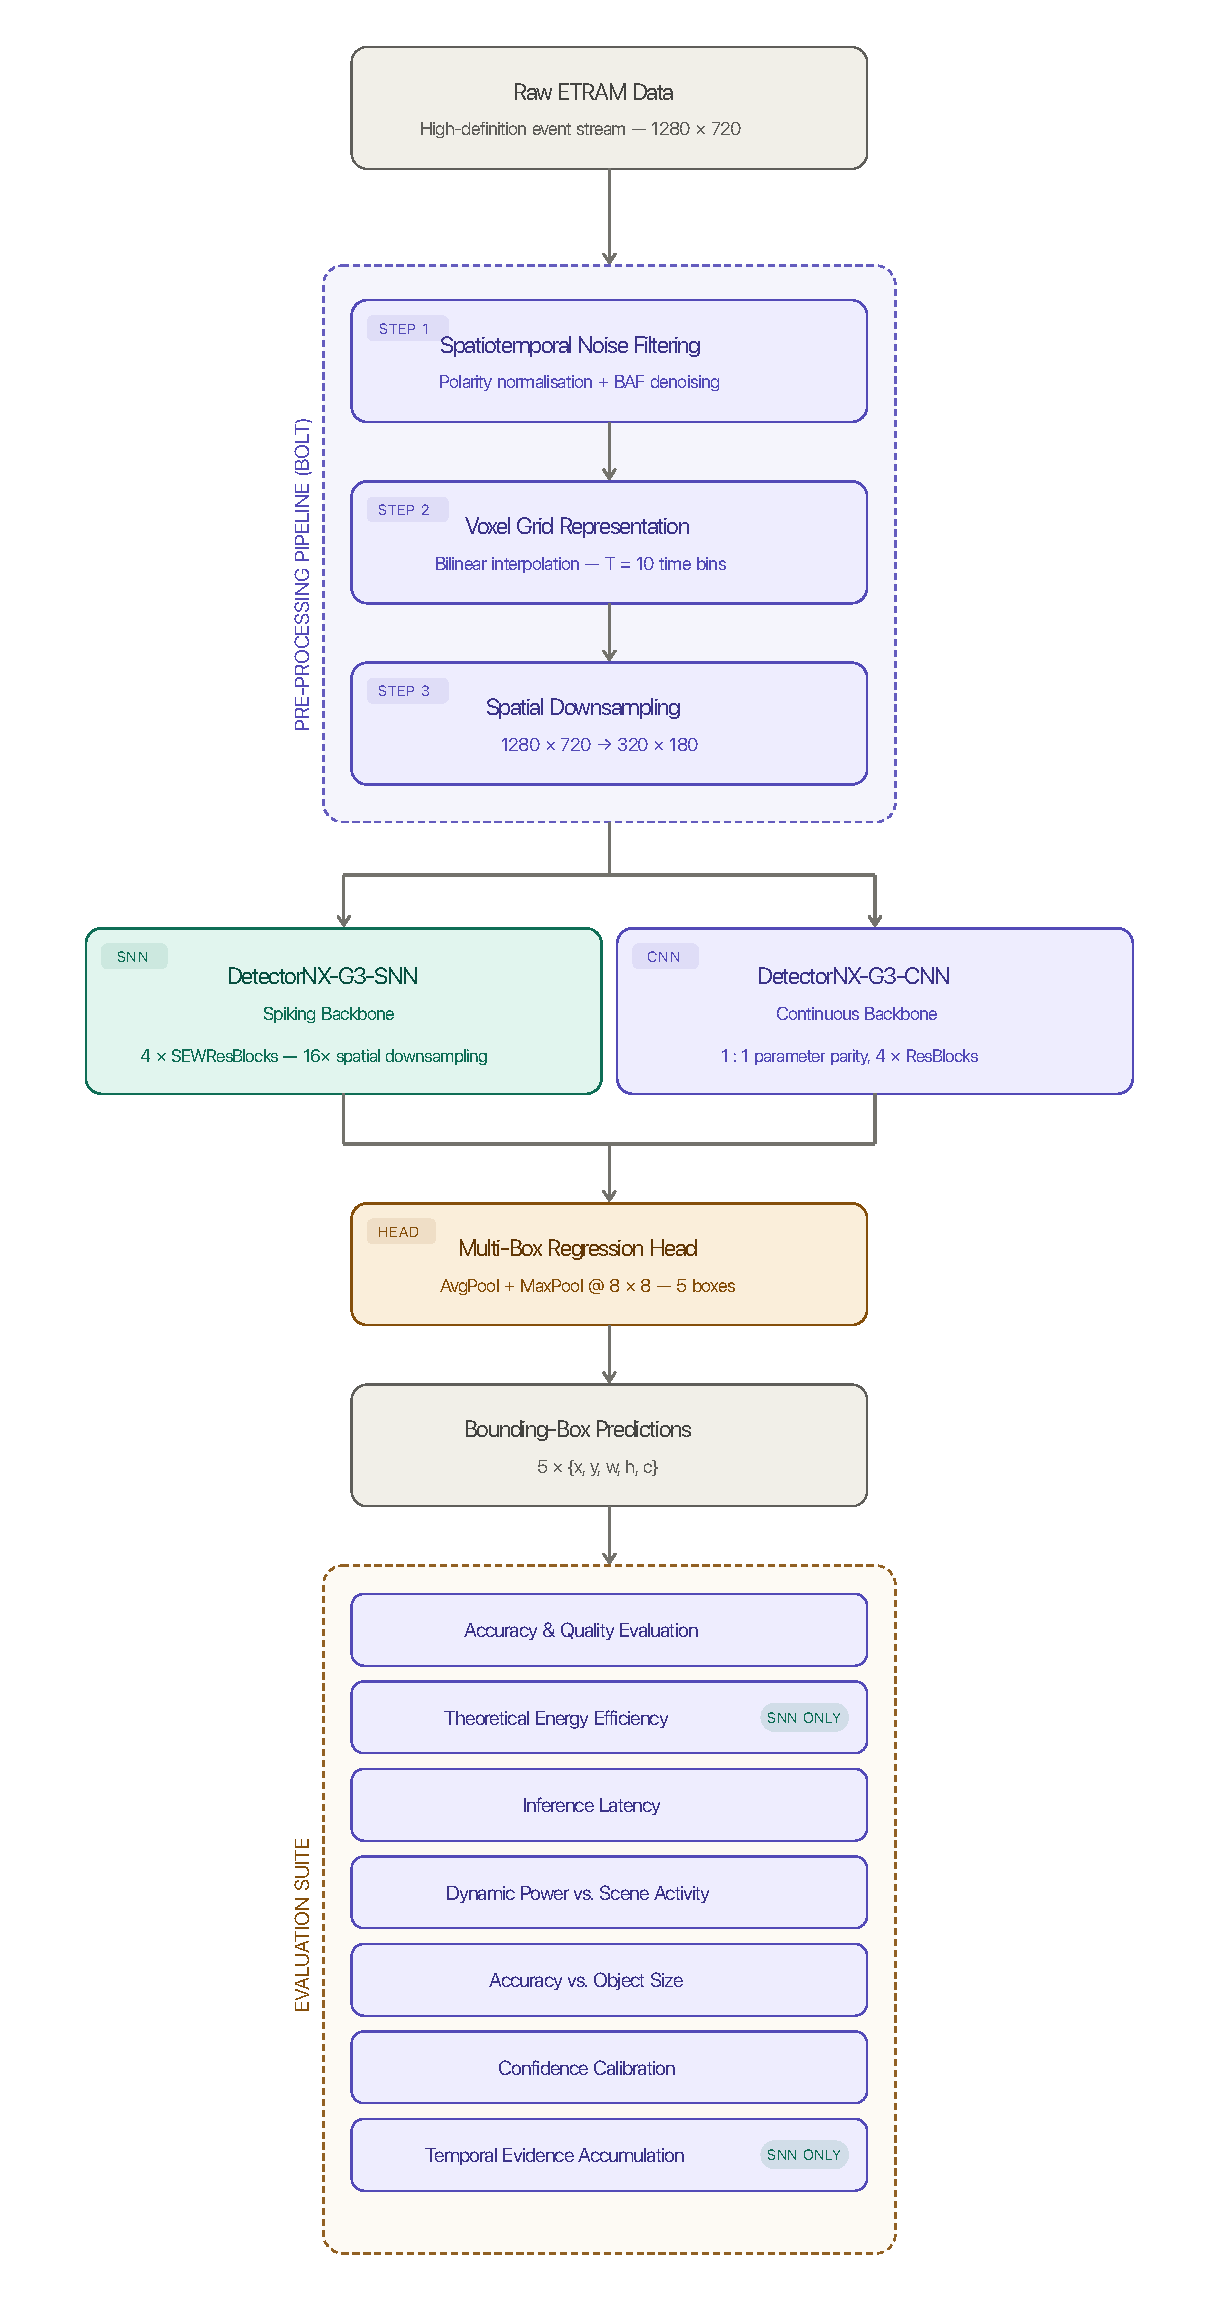
\includegraphics[trim=0 0 0 0, clip, width=0.95\textwidth]{chapter_3/figures/high-level-architecture.pdf}
    \caption[High-level system architecture pipeline.]{The high-level system architecture pipeline, illustrating the flow from raw ETraM high-definition event data, through the fixed REPLICA preprocessing stages, into the interchangeable neural backbone (SNN or CNN), and concluding with the multi-box regression head and the comprehensive evaluation suite.}
    \label{fig:system_architecture_block}
\end{figure}

As illustrated, the architecture is divided into four primary sequential stages, where the central neural backbone acts as an interchangeable module:

\begin{enumerate}
    \item \textbf{Data Ingestion \& The REPLICA Pipeline (Fixed):} 
    Raw, asynchronous event data at a high spatial resolution of $1280 \times 720$ is ingested from the ETraM dataset. 
    Due to the conventionally sparse and noisy nature of neuromorphic hardware outputs, the data enters the \textit{REPLICA} preprocessing pipeline, which is heavily adapted from the methodology proposed in the original ETraM study \cite{Verma_2024_CVPR}.
    While the core spatiotemporal noise filtering and bilinear temporal interpolation (to $T=10$ bins) remain faithful to the original study, this project included an additional spatial downsampling stage ($ds=4: 1280 \times 720 \rightarrow 320 \times 180$).
    This modification was strategically implemented to ensure training feasibility on local accelerator hardware and reduce input sparsity, thereby improving the stability of neuronal feature extraction.
    This stage is detailed thoroughly in Section \ref{sec:data_processing}.

    \item \textbf{The Neural Backbone (Interchangeable):}
    The preprocessed output of the \textit{REPLICA} pipeline serves as the input to the primary feature extraction engine.
    This stage houses either the spiking architecture \texttt{SNN\_MAX\_REPLICA\_SE} or its exact continuous counterpart, \texttt{CNN\_MAX\_REPLICA\_SE}.
    Both backbones utilize four functional blocks incorporating Squeeze-and-Excitation (SE) mechanisms and Residual connections (\texttt{SEWResBlock}) to extract deep semantic features while performing an aggressive $16\times$ total spatial downsampling. 
    The evolution and formal design of these backbones are detailed in Section \ref{sec:model_design}.

    \item \textbf{Multi-Box Regression Head (Fixed):} 
    The final abstracted feature maps from either backbone are fed into a unified detection head. 
    To resolve the spatial ambiguities and ``ghost detections'' observed in earlier architectural iterations, the head utilizes an $8 \times 8$ Adaptive Pooling mechanism to aggregate features from 64 spatial receptive blocks.
    This abstracted information is then mapped to a final output tensor of shape $[B, 5, 5]$, representing the top 5 predicted bounding boxes per image. 
    Each detection is defined by the feature set $\mathcal{F} = \{x, y, w, h, c\}$, where $(x, y, w, h)$ denote the normalized bounding box coordinates and $c$ represents the object confidence logit.
    The regression output is evaluated via a fully vectorized Multi-Box Loss function during training.

    \item \textbf{Evaluation \& Benchmarking Suite (Fixed):}
    The predictions and internal neuronal activity from the models are passed into a specialized benchmarking suite. 
    This stage is responsible for the rigorous empirical comparison of the two architectures across five distinct dimensions: real-time dynamic power consumption, accuracy variations relative to object size (addressing the inherent ``quantization error'' in SNNs \cite{cordone2022objectdetectionspikingneural}), model confidence calibration, temporal evidence accumulation, and latency observed on local hardware. 
    These metrics were specifically selected to satisfy the project's success criteria and provide a comprehensive evaluation of the neuromorphic paradigm. This standardized evaluation framework ensures that the findings are scientifically robust and reproducible. This benchmarking suite is detailed thoroughly in Section \ref{sec:experimental_setup}.

    \todo[inline,backgroundcolor=myblue,textcolor=white]{Re-write this section, and link it to the Success Criteria from Introduction.}

\end{enumerate}

Using the modular pipeline guarantees that the SNN and CNN variants are evaluated identically, receiving the exact same preprocessed event volumes and outputting predictions through an identical regression and benchmarking framework.